\section{Introduction}

The merger of survey data with administrative data has grown more popular recently, as researchers seek to lower data collection costs, reduce the questionnaire length and improve data quality. However, consent of the respondents is usually needed to merge administrative data and survey data. Because of the utility of linked administrative and survey data, the consent for linkage question has been the focus of much research into its wording (SAKSHUAG PAPERS AND OTHERS) and placement. \cite{Sakshaugetal13} have shown that placing the question at the beginning of the questionnaire collects more YES responses than placing at the end (xy\% vs yz\%), and this approach is catching on among surveys (A FEW SURVEY HERE THAT DO BEG PLACEMENT, WOULD BE GREAT TO FIND THOSE THAT HAVE *MOVED* THE QUESTION -- MAYBE PASS?). 

We worry, however, that asking the linkage consent question at the beginning can alter the way respondents answer later questions in the survey. CITES HERE ON THE FACT THAT ONE QUESTONS CAN AFFECT OTHERS (SCHWARZ, ORDER EFFECTS) \cite{McFarland81}. 

We have two competing hypotheses about how consenting at the beginning of the survey interview could affect responses. The \textit{worse-respondent hypothesis} holds that respondents who grant consent at the beginning of the survey are not motivated to provide high quality responses int eh rest of the survey, because they think that their responses will be usurped by administrative data. The \textit{better-respondent hypothesis}, on the other hand, holds that those who consent at the beginning are \textit{more} motivated to answer correctly because they believe that their responses may be checked against administrative records, and that there may be consequences for misreporting. 

Because surveys which want to increase their consent rates are asking the consent rate at the beginning of the survey, it is important that we understand the effects of this question on survey data quality. If the better respondent hypothesis holds, then asking the linkage consent question at the beginning not only maximizes the consent rate, but it also reduces measurement error. If the worse\--respondent hypothesis holds, however, surveys face a tradeoff between a high consent rate and  measurement error. In addition, several methodological studies have used administrative data to study measurement error in survey responses, and the experimental surveys underlying these studies have relied on consent questions asked at thE beginning of the survey (\cite{Kreuteretal10,Kreuteretal14}) \cite{Eckmanetal14} \cite{Eckmanetal15b}). If these experiments are not representative of usual survey response behavior due to effects of the linkage question itself, we should be vary of their results. For these reasons, we investigate our two competing hypotheses about a connection between linkage consent and measurement error.


\section{Background}

MOVE SOME OF THIS UP:

Several studies have identified the design features of the linkage question that leads to high consent. One way to do this is to adjust the wording of the question. Studies show that an indirect (Opt-Out) consent has a positive effect on the consent rates (\cite{Batesetal05}, \cite{Pascale11}, \cite{Dasetal14}), but many respondents do not seem to understand the subtleties of the question (\cite{Batesetal05}), so it is hard to argue that this is a good method to obtain consent. Another design features survey methodologists can account for is the selection of interviewers. But influential interviewer characteristics vary from study to study (see \cite{Beste11}, \cite{Sakshaugetal13}, \cite{Salaetal10}).

Another parameter that affects consent rates is the placement of the administrative data linkage question. Studies often put the administration data linkage question in the back of the questionnaire, because it is seen as sensitive. And as we see in the literature sensitive questions often placed in the later stage of the interview to lower break-off or unit nonresponse rates (\cite{Cantoretal02}, \cite{Sudmanetal82}, \cite{Tourangeauetal07}). In most of the American surveys the administrative linkage question is at the end, but actually it is better to place the administration linkage question at the beginning to get higher consent rates (see \cite{Sakshaugetal13}).

To explain the change in respondents behavior we use the terms Optimizer and Satisfier proposed by Krosnick (1991). Optimizers are respondents who put a high effort and diligence in answering the questions in an interview. Satisfiers on the other side put the least effort into the interview process. Those are the respondents who are inattentive as reading or hearing the question or ignore further introductions. They may skip stages of the cognitive response process or do not recall all information needed and just use the least effort to give a plausible answer.

Optimizers and Satisfiers are both the termini of a continuum (\cite{Krosnick99}). Both are ideal types and should not exist in their full might; at least there should be very few of these extreme types. Anyway every respondent is located somewhere on this continuum.

The basic attitude (beliefs, values and goals) that determines the initial location on the optimizer-satisfier-continuum should be stable for each respondent in the pre-interview situation. Also we assume that the basic attitude determines the effort that respondents put in the cognitive response process. With the consent to participate in the interview, the respondent is exposed to several cues like interviewer characteristics and questionnaire design that should motivate most of the respondents to move from their initial location. We hypothesize consenting to the administrative data linkage question at the beginning of the interview changes the motivation of the respondents so that they leave their initial location on the optimizer-satisfier-continuum. In this sense, the linkage question can be seen as a treatment. The question is if the effect of this treatment is perceptible in the data and in which direction it goes, because respondents can be motivated to give better responses or they could give worse responses. It is not clear how the administrative data linkage question motivates the respondents to move on this continuum, but a general tendency should be perceptible if we aggregate responses.

There are two different ways how the treatment effect of the administrative data linkage question can affect survey measurements. For one if the administrative linkage question is asked at the beginning of the interview, respondents could think that with the administrative data linkage incorrect data can be corrected. If they do so, they would take less care in their response and whether these are wrong (worse-respondent hypothesis)\footnote{A similar effect might occur with the interviewers: They could also believe that if they have the consent of the respondent, they do not need to read the questions accurately, because it may be corrected afterwards (worse-interviewer hypothesis) -- but we do not investigate this here.}. On the other hand, those who consent may be better respondents, because they believe that their responses may be checked, and think they may get in trouble if they are found to be lying (better-respondent hypothesis). This study tests the worse-respondent hypothesis against the better-respondent hypothesis. These hypotheses lead to the main research purpose: to evaluate if the consent to the administrative data linkage question leads to a trade-off between a high consent rate and a possible measurement error or if this placement design leads to a win-win situation as higher consent rates can be obtained and measurement error can be lowered.

%The cognitive process of answering a survey question has four steps: a) Comprehension, b) Retrieval, c) Estimation and Judgment and d) Reporting (\cite{Tourangeauetal00}, \cite{Dillmanetal09}, \cite{Grovesetal09}). In the first step -- comprehension -- the respondent is encoding and interpreting the question in the survey context and tries to figure out what exactly is wanted from him/her. In the retrieval step, the respondent tries to remember the information that is important to answer the question, such as facts, memories, events and so on. When the respondent is in the state of Estimation and Judgment, (s)he is thinking if the retrieved answer is right, accurate enough or can be mentioned in the context of the interview. At the end of the process reports his/her answer.

%The response process is not necessarily linear but a process that can skip stages and contains overlaps between the stages. In fact many things can go wrong. In the comprehension process. Respondents may not notice introductions to the question or do not bother to read them. Further they can run across unfamiliar terms or the question requests detailed information that the respondent does not have. One major problem in asking questions is the different meaning that researchers and respondents have about a specific term (\cite{Tourangeauetal00}).


\section{Data Sources}
To test our two compting hypotheses, we exploit a data set that combines responses from a telephone survey and administrative data. The link to administrative data lets us caclulate measurement error and test the effect of granting linkage consent at the beginning of the survey on response accuracy.

\subsection {Survey data}\label{sec:survey}
The Institute for Employment Research conducted a survey in Fall 2014 to investigate different methods of protecting individual privacy and transferring selected addresses to a data collection contractor (See CITE KREUTER SAKSHAUG TOURANGEAU IN NEW JSSAM ISSUE for results of the wording experiment (PLACEMENT TOO?)). Luckily, for our purposes, this survey also contained a consent experiment that we can exploit to test our hypotheses. The selected sample contained 7,183 persons selected from administrative records. 1,034 cases completed the telephone survey, which took place from October to December, 2014.\footnote{Nonrespondents were then approached for a web survey, but we do not data from the web survey in this investigation.} The response rate is XY\% (APPOR RR1). CITE FOR AAPOR RR NEEDED. GEORG -- FILL IN RR HERE

\texttt{Why 1034 here? does not match 1208 or 1128 given below. LET'S REVIEW THESE NUMBERS TO MAKE SURE THEY'RE THE ONES WE WANT}

The survey contained three fully-crossed experiments. Two experiments were designed to evaluate the effects of wording and placement of the administrative data linkage question on consent rates. Approximately half of the respondens were asked at the beginning ofthe survey (n=611) and half were asked at the end (n=592). The wording experiemnt on this question involved gain versus loss framing, where gain framing is XYZ and loss framing is ABC. Table \ref{tab:consentrates} shows that linkage consent rates were higher when the question was asked in the beginning, as shown in previous studies. The table also shows that the wording experiment did not significantly affect consent rates in the telephone survey. FOr more analysis of these two consent experiments, see CITE.

\texttt{911 + 592 = 1203 -- ??}


\begin{table*}
\begin{threeparttable}[b]
\caption{Linakge Consent Rates by Experimental Condition, in \%}\label{tab:consentrates}
\begin{tabular}{l.{3}.{3}.{3}}
\toprule
&Gain Frame & Loss Frame & n \\
\midrule
Asked in beginning	& 90.8 &90.5 &611 \\ 
&		(1.6)& (1.7)&       \\ \addlinespace
Asked in end        &79.2  &81.5 &592 \\
		&(2.3) &(2.2)&    \\ \addlinespace
n		&595	&608 &1203  \\ \addlinespace
\bottomrule
\end{tabular}
\vspace{.5em}
\begin{tablenotes}\small
		\item Note: Standard errors in parentheses 
	\end{tablenotes}
\end{threeparttable}
\end{table*}

ADD \%S TO ROW AND COLUMN TOTALS (AND STDERR)

The survey contained an additional experiment, fully crossed with the two consent experiments, that we do not exploit for this analysis but which warrants mention. Before the survey started, cases were randomly divided into two groups: an Opt-Out group and a control group. (This experiment was fully crossed with the consent quetsion wording and placement experiments). Opt-Out group was mailed a letter describing the telephone survey and given an opportunity to refuse the transfer of their contact inforation data to the survey firm by returning a postcard. Those who did not return were postcard were assumed to have given their consent. The contact information for cases in the control group was passed to the survey firm in the usual way, with no opportuity to refuse. This experiment was mandated by XYZ MORE HERE, and also included an Opt-In group, but due to small sample sizes and concerns about selection bias among this group, we drop this group from  our analysis data set. For more details on this experiment, see CITE SAKSHAUG PAPER. 

In the Opt-Out group 42\% of the 5,000 selected people refused take part. MORE HERE TO CONVINCE READER THAT GAIN/LOSS AND OPT-OUT/CONTROL NOT A PROBLEM

The questionnaire included questions on XYZ. Several of these questions match concepts in the administrative data and thus we can calculate measurment error in these variables.

We also have access to paradata for this survey, including interviewer characteristics and call record data. 

\subsection{Administrative data}\label{admin}
With respondent permission, We can link the survey data described above to administrative data held by the German Federal Employment Agency to get additional variables for our analysis. The administrative data used for this study come from the Integrated Employment Biographies data set (IEB), which contains complete employment biographies of working-age persons: employment, receipt of two types of unemployment benefits and participation in active labor market programs. The data also contain personal characteristics such as date of birth, vocational training, nationality, gender and residence (\cite{Fitzenbergeretal05}). For this study, we use data from December 2014, which matches the field period.

The data are used by the Federal Employment Agency to calculate social security and unemployment insurance payments (see FDZ-Methodenreport 13/2014:6). NEED BIBTEX CITE HERE. For this reason, variables related to employment duration and receipt of unemployment benefits are of high quality, and those which are tendential to the administration of these programs (such as nationality and education) are of lower quality (CITES NEEDED -- FITZENBERGER?). As discussed below, we at times had to impute missing values in the administrative records. 

Because the sample was selected from the same administrative data set that we are linking to and we have a unique identifier for each respondent, linking is rather straightforward, and we use exact linkage rather than statistical matching. However, we did encounter a few issues that caused us to drop some cases at the linking step. First, not all respondents consented to linkage of survey responses with administrative data (n=178) and we were not allowed to link those cases. Second, some respondents provided a gender or date of birth in the survey that did not match the records (n=19), leading us to think we may have spoken to the wrong family member. Third, others reported that they were government officials or self-employed; because these employment spells are not captured in the administrative data, we drop these respondents as well (n=38). Fourth, we drop cases where the administrative records are incomplete -- MORE DETAILS HERE, HOW MUCH MISSING DATA TRIGGERED DROPPING? (n=31). From the 1,208 cases that completed the telephone survey, we were able to link 1,128 of them and these cases form the basis of our analyses.\footnote{Note that the numbers appear not to sum because tehre are some cases that appear in more than one problem category.}

THESE NUMBERS DO NOT MATCH SECTION 3.1


\section{Treatment Effect Estimation Methods}\label{method}

The linked survey and administrative data allow us to calculate measurement error in respondent reports and thus test our hypotheses. $\epsilon_{j,i}$,  measurement error in question $j$ for respondent $i$, is:

\begin{equation}
\epsilon_{j,i} = \text{response}_{j,i} - \text{admin}_{j,i}
\label{eq:hyp_epsi}
\end{equation}

However, we cannot simply compare the average measurement error among those who granted linkage consent at the beginning of the questionnaire with those who did so at the end, because the two sets of consenters are not equivalent.  Although assignment to the beginning and end experimental groups was random, the cases who consentd at the beginning are somewhat different than those who consented at the end (as we can see already in the differing consent rates in Table \ref{tab:consentrates}. 

The most appropriate control group for our research question is a set of respondents who were \textit{not} asked at the consent question at the beginning, but who \textit{would have given consent, had they been asked}. This group of course does not exist, but we can use statistical techniques to approximate it, taking advantage of the placement experiment in this survey. We use entropy balancing to derive weights that balance the observable characteristics of those who consented at the beginning and those who consented at the end. 

Note that we cannot use the nonconsenting cases in our analyses, because we cannot calculate $\epsilon_{j,i}$ for the nonconsenters.

Entropy balancing is a technique developed by \cite{Hainmueller12} to achieve balance between treatment and control groups. Unlike earlier propensity score reweithing approaches, which first estimate a treatment propensity and then develop weights from teh estiamted propensity scores (CITE), entropy balancing takes a more direct approach. The technique imposes constraints on the first, second and third moments of the distributions of the observable characterists and then solves for weights that meet those constraints (\cite{Hainmueller12}). For example, we might require that all means (the first moment) differ by less than 1\% on all variables and the variances (the second moment) by less than 10\%. For this study we constrain only the first moment, the mean, which increases the likelihood the the method converges and is often sufficient to balance out the variance and skewness of further moments too (\cite{Hainmuelleretal13}).

After developing a set of weights that balance the two sets of cases, we use these weights to test whether average measurement error is larger among the treament cases (worse-respondent hypothesis: $\bar{\epsilon}_{treated} > \bar{\epsilon}_{control}$) or smaller (better-respondent hypothesis: $\bar{\epsilon}_{treated} > \bar{\epsilon}_{control}$).

This appraoch to estimating treatment effects, like the earlier propensity score approaches, relies on three assumptions. First, the Stable Unit Treatment Value Assumption  Assumption (SUTVA), that the cases are independent and the effect of the treatment on one case does not depend on who else is in the treatment group (Rubin80, Holland86 FIX THESE CITES). This assumption should be satisfied in a telephone survey where the cases do not interact, but very strong interviewer effects in the consent question could be an issue here (\cite{Beste11}, \cite{Sakshaugetal13}, \cite{Salaetal10}). For this reason, we do control for some interviewer characteristics, as discussed below. Second, the overlap assumption requires that the treatment and control cases contain persons with similar characteristics, on both observed and unobserved variables (\cite{Heckmanetal98}). For example, it should not be the case that all persons who concented at the beginning support the Social Democrats and no persons who consented at the end do. This assumption should be met in this study because the initial allocation to the beginning and end experiments was random. 

Third, the conditional independence assumption holds that balancing the observed variables is sufficient and also balances all relevant unobserved variables (\cite{Imbens14}). This assumption, also called strong ignorability (\cite{Stuart10}), is fundamentally untestable (\cite{Imbens04}). The best we can do is argue that we have included as many variables as possible, what \cite{Stuart10} calls the ``kitchen sick'' method.

We apply the entropy balancing model to X variables derived from the administrative data, survey paradata and from random assignment to experimental conditions (Table \ref{tab:covariates}). From the administrative data we have both demographic characteristics as well as  variables related to respondents' labor market history. We include indicators of the two experiments not involved in the construction of our treatment and control groups: the consent question wording experiment (gain vs loss framing) and the two methods of transfering addresses to the data collection contractor (opt-out vs control).\footnote{As discussed in Section \ref{sec:survey}, we drop all cases in the Opt-In condition, due to concerns that people who opt-in to a survey have different survey response behavior. We also note that no other surveys use this recruitment method and thus the results of that experiment do not generalize to other environments.} We also use four interviwer characteristics and two variables from the call record data set. 

In developing the entropy balance weights, We do not use the survey data themselves, because our research question concerns whether and how treatment (consenting to the linkage question at the beginning of the survey) changes survey responses. If we were to balance the treatment and control groups on variables in the survey data, we would remove some of the treatment effect that we wish to estimate. Following advice from \cite{Rosenbaum84}, \cite{Frangakisetal02}, \cite{Greenland03}, \cite{Caliendoetal08}, and \cite{Stuart10}, we exclude from our balancing approach any variable that is affected by the treatment of interest and use only variables that are time invariant or measured before treatment. 

\renewcommand{\arraystretch}{0.8}
\begin{table*}[h]
 \caption{ Variables used for the entropy balance model}\label{tab:covariates}
\begin{tabular}{lll}
  \addlinespace \toprule\addlinespace
\textbf{administrative data} &Sociodemographics &  Gender\\ \addlinespace
&							&Year of birth \\ \addlinespace
&							&Education\\ \addlinespace
&							&professional education\\ \addlinespace 
&							&West/East Germany\\ \addlinespace			
&Labor market history				& Share of different employers\\ \addlinespace 
&							& Mean duration, Total duration  \\
&							& and Number of spells \\ \addlinespace
&							&  \ \ \ - UBII receipt   \\ \addlinespace
&							&  \ \ \ - UB I receipt \\ \addlinespace
&							& \ \ \ - ALMP participation \\ \addlinespace
&							&\ \ \  - Employment\\ \addlinespace
&							& \ \ \ - Unemployment \\ \addlinespace
&							& \ \ \ - Job seeking \\ \addlinespace \addlinespace
 \midrule \addlinespace
\textbf{Sample}&						&Sample Experiment \\ \addlinespace
 &							&Loss/Gain-frame experiment \\ \addlinespace \addlinespace
 \midrule \addlinespace
\textbf{Interviewer variables}  &			&Age\\ \addlinespace
(CATI only)&							&Gender\\ \addlinespace
&							&Experience\\ \addlinespace
&							&Education\\ \addlinespace \addlinespace
 \midrule \addlinespace
\textbf{Call record data}	 &				& Number of contacts\\ \addlinespace
 (CATI only)&							& Contact time\\ \addlinespace
 \bottomrule
 \end{tabular}
\end{table*}

To test if the covariates are balanced, we compute the standardized mean differences GIVE FORMULA HERE. A standardized mean differences greater than five percent in one more is a sign that balance has not been achieved (\cite{Caliendoetal08}). 

\subsection{Treatment Effect Estimation}

To estimate the treatment effect we use simple regression models where the dependent variable is $\epsilon_{j,i}$ and the sole independent variable is the treatment indicator ($0$ for cases in the control group, $1$ for those in the treatment group). We apply the weights from the entropy balance model and estimate robust standard errors to protect against heterogeneity. If our weights balance the treatment and control group on all observed and unobserved characteristics such that the only remaining difference between them is treatment itself, then the coefficient on the treatment effect indicator is our estimate of the effect of giving consent at the beginning of the survey on later measurement error. A positive coefficient is evidence for the better-respondent hypothesis, and a negative coefficient is evidence for the worse-respondent hypothesis.

We can calculate measurement error for all variables that are in both the survey and the administrative data. These variables are given in Table X.  Many of the variables for which we calculate measurement error are dichotomous or categorical and thus measurement error $\epsilon_{j,i}$ is best mesaured as an indicator of error: $I(\text{response}_{j,i} \neq \text{admin}_{j,i})$. These variables are flagged in the third column of Table X. \textbf{Table X also shows that the number of cases available for each variable change, due to skip patterns and missing data.} For each set of cases, we rerun the entropy balancing technique and create new sets of weights. Question text and notes about how the survey and administrative variables were coded are given in Appendix A.


\section{Results}

Intro here

\subsection{Testing balance}
Figure \ref{fig:balance} shows the weighted and unweighted standardized mean differences between the treatment and control group for the variable misreport in employment status. As mentioned, before the means should not differ more than five to be recognized as balanced (\cite{Caliendoetal08}). As we can see in our example, 25 of 47 variables in the model have higher standardized mean difference than five percent before balancing. With the entropy balance method, we can balance these to nearly zero for each covariate. Therefore the model accomplishes his purpose.

Unfortunately not all the analysis variables could be balanced out. Table \ref{tab:achieved_balance} (p. \pageref{tab:achieved_balance}) shows the 14 variables and the summarized standardized mean differences from the CATI and web data. The column of interest is the third and seventh: number of standardized differences \textgreater5 after weighting. As the guideline is that the standardized mean differences should be smaller than five (\cite{Caliendoetal08}) the entropy balance scheme failed for all variables that have at least one difference greater than five. For the CATI data the variable misreport in employment status for the respondents who stated non-employment could not be balanced out. Therefore we cannot calculate the average treatment effect for this one variable in the CATI data.

We can see some differences in the web data. In the CATI data the highest deviation and the mean bias after weighting is nearly zero in most cases. For the web data the entropy balance scheme does not work as good. For the employment variables we can see that we have a standardized mean differences that differ from zero. Still the highest deviation for the employment variables is still smaller than five so that we can account these as balance achieved. Again we cannot achieve balance for the variable misreport in employment status for the respondents who stated non-employment. But the reason for that is because all respondents in the web survey stated that they are employed. Also, for the web data it is not possible to achieve balance for the variable income because 14 covariates have standardized mean differences above 5.

The reason why the model did not work could be that the number of cases are insufficient as at the same time the differences in distribution over the discrete covariates are too big.

A possible solution could be to stepwise take out the covariate with the highest standardized mean difference and include it to the regression model. In the next step the treatment effect could be analyzed in the context of the unbalanced covariates. The problem is that the share of unbalanced covariates is really high (see Table \ref{tab:achieved_balance}) and therefore we would have blown up regression models. Further most of the covariates are not really interpretable as they were calculated to predict a propensity (see \ref{covar} Covariate for balance, p. \pageref{covar}).

If we compare the achieved balances in both modes, it seems like in the CATI data the entropy balance works pretty or in no sense. Every time when balance is achieved the standardized differences go not over 0.1. In the web survey the entropy balance model does not achieve such good results. The standardized mean differences stay less or equal five, but scatter more in the range of five and zero than in te CATI data. This suggests that the selection bias between consenters in the begin and end is higher in the web survey.

\newpage
\begin{figure}[b]
\caption{Standardized Mean Differences before and after Weighting (n=736)}
\centering
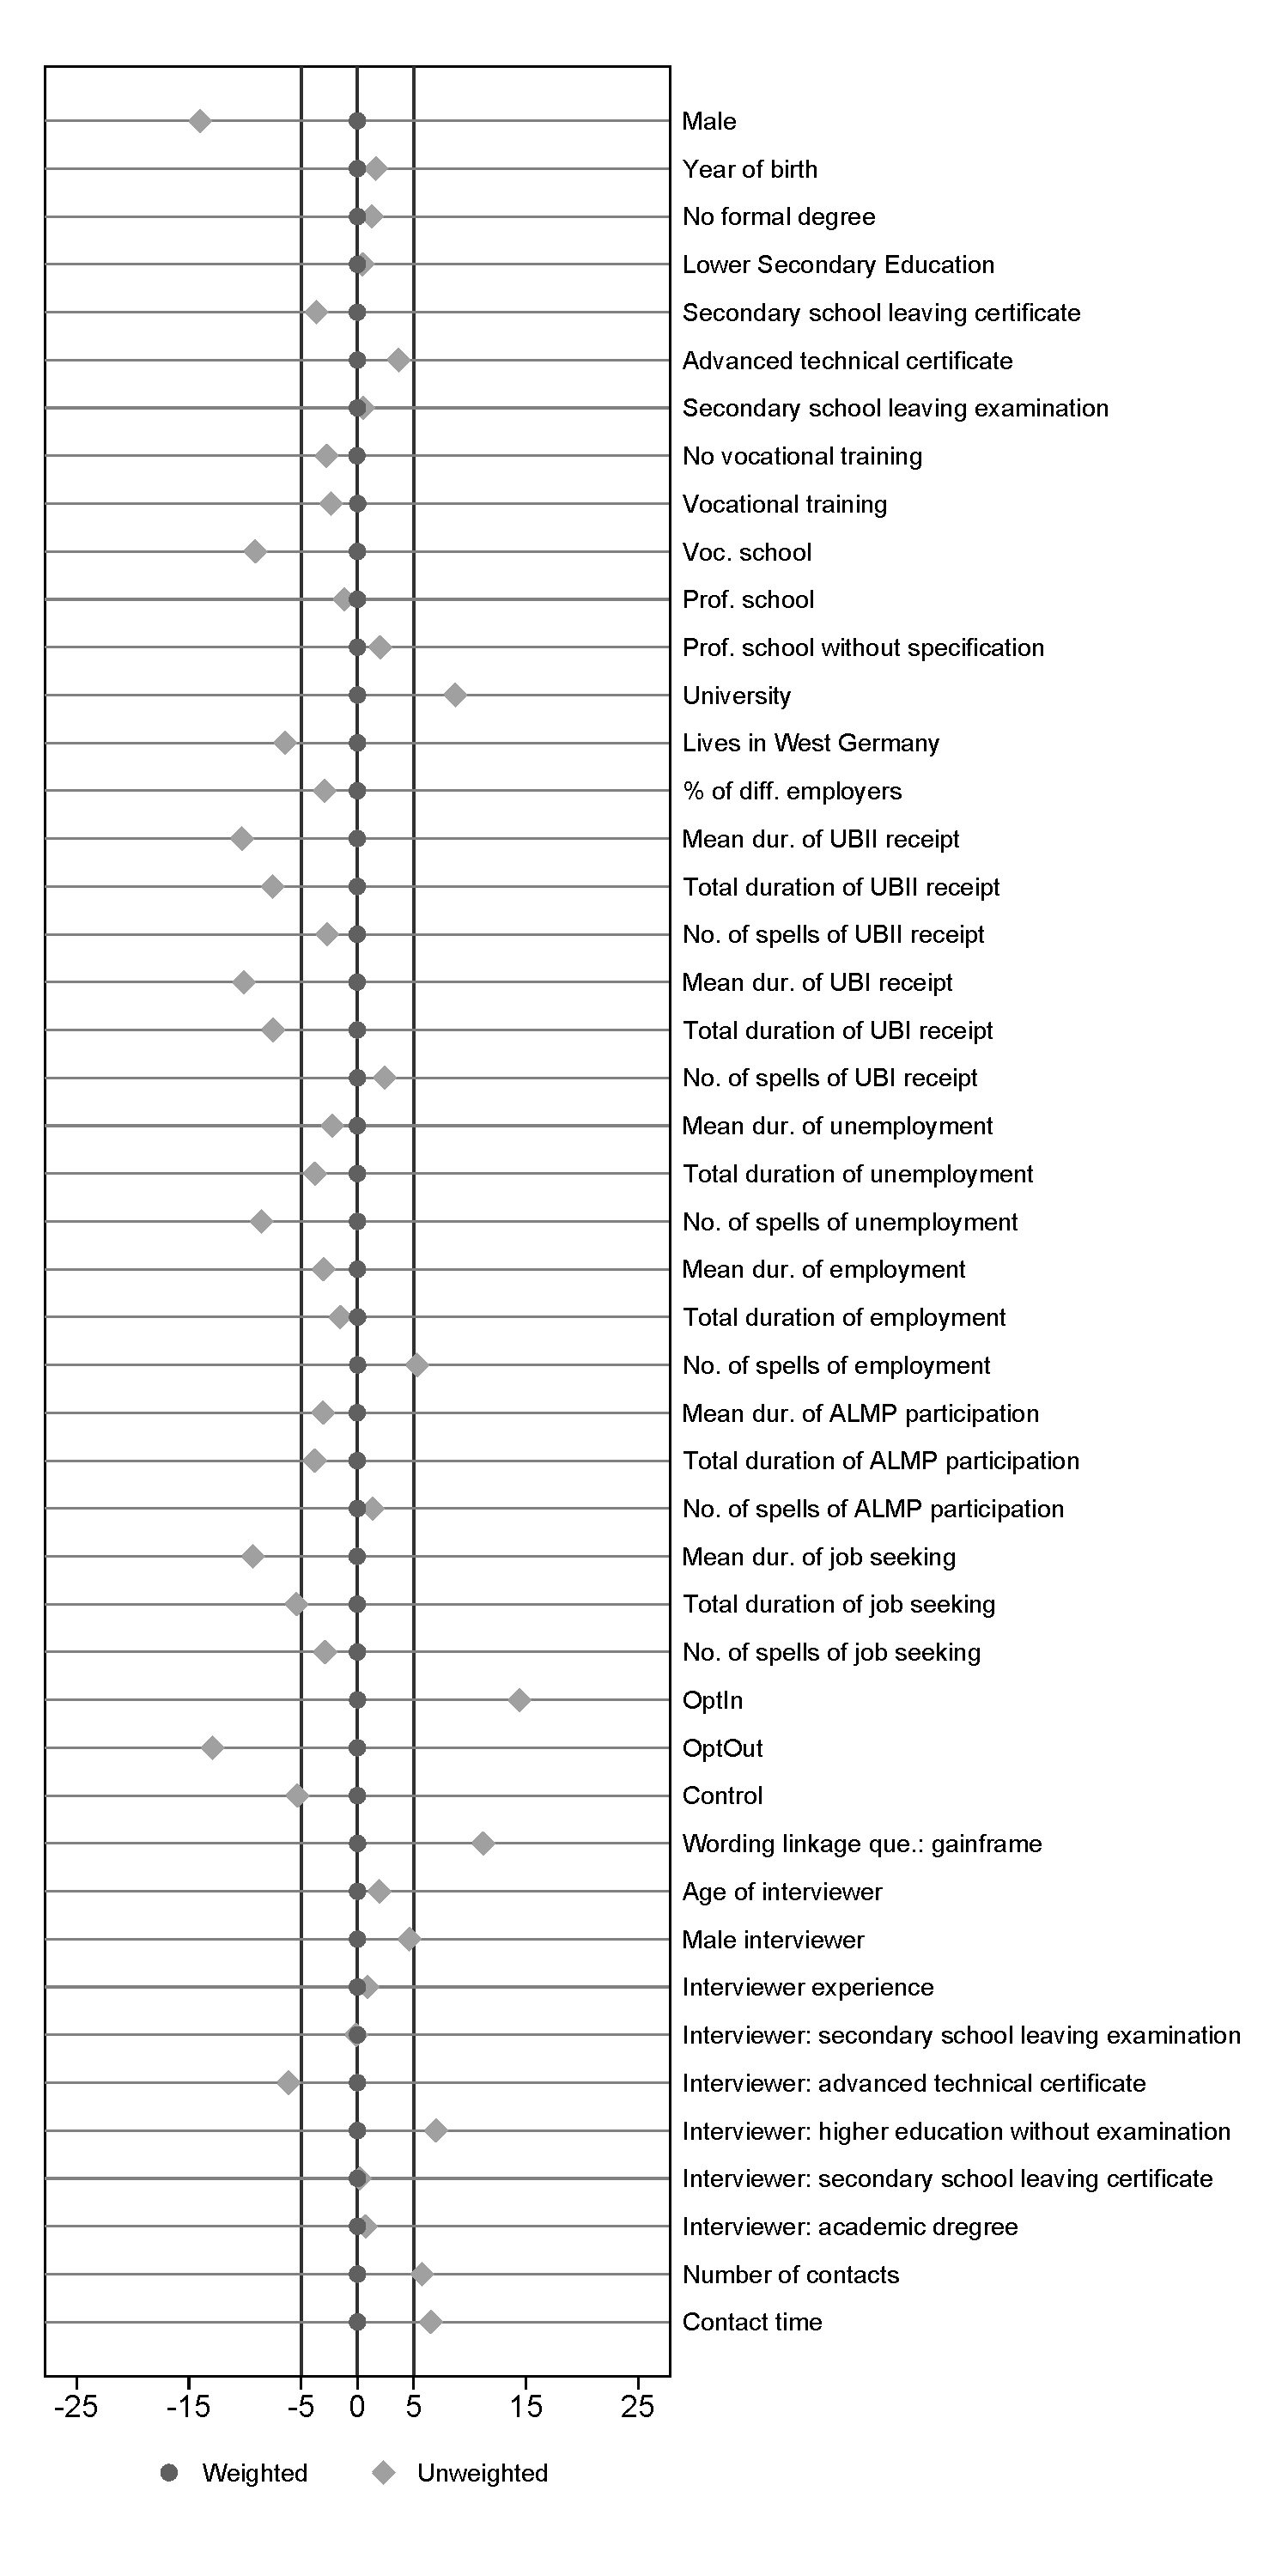
\includegraphics[scale=0.4]{balance.pdf}
\label{fig:balance}
\end{figure}

\newpage
\begin{threeparttable}
\caption{number of variables with standardized differences \textgreater 5, highest deviation and mean bias for standardized mean differences after applying the entropy balance model}
\label{tab:achieved_balance}
\begin{tabular}{p{5cm}p{1.5cm}p{1.5cm}p{1.5cm}p{1.5cm}} 
\cmidrule(r{0.25em}){2-5} 		
\textit{employment status} &	number before weigthing	&	number after weighting	&	highest deviation after weighting	&	Mean bias after weigthing \\	
\midrule
Error indicator	&	25	&	0	&	0.0	&	0.0	\\
Error indicator - stated employed	&	29	&	0	&	0.0	&	0.0		\\
Error indicator - stated unemployed	&	42	&	28	&	23.2	&	5.8	\\
\addlinespace
\textit{Start Date of Employment Spell}	\\
Minimum Deviation from true date	&	29	&	0	&	0.0	&	0.0	\\
Item Nonresponse	&	24	&	0	&	0.0	&	0.0	\\
\addlinespace
\textit{wage variables}	\\
Income	&	34	&	0	&	0.0	&	0.0	 \\
Item Nonresponse	&	27	&	0	&	0.1	&	0.0	\\
\textit{Error indicator for citizenship}	&	25	&	0	&	0.0	&	0.0 \\
\end{tabular}
\vspace{.5em}
    \begin{tablenotes}\small

    \end{tablenotes}
\end{threeparttable}




\subsection{Treatment Effects}

In Table \ref{tab:tab_estimates} we can see the average treatment effects of the treated (ATT) that consent to the administrative data linkage question has on our selected variables. In contrast there is the estimation without the balanced covariates referred to as naive estimation. To get the average treatment effect and the naive estimation, a simple regression was used. Misreport in employment status is a binary coded variable (\(0=true\ report, 1=false \ report\)). Therefore we see the change of proportion that comes with the treatment. For example the treatment effect of 0.02 is a change of two percentage points through the treatment of consenting to the linkage question at the beginning of the interview. That means due to the administrative data linkage question 15 (out of 736) more people misresport their employment status. This effect, if true, would support our worse-respondent hypothesis: the error due to the linkage question increases. On the other sid a negative coefficient would support the better-respondent hypothesis.

For the misreport in employment status we have an effect of two percentage points. This result does not change whether we use an estimation with balanced covariates or an unadjusted estimation. This suggests that balance is not necessarily needed for estimate the average treatment effect.

If we take a deeper look and differ the misreport in employment status into the ones that stated that they have an employment and those who stated that they were non-employed, we can see that the treatment effect for the people who stated that they are employed decrease to one percent point for the balanced estimation and two percent points for the the naive estimation. Again we see that the standard errors are bigger than the estimation itself and we can not make out a real direction of the treatment effect because the result can be in the negative and positive range. And also the non-significances show that there is no effect.

For the respondents who stated that they were unemployed we have a high rate of misreports of nearly 50 \%. One possible explanation could be that side-jobs or mini jobs are not really considered as jobs. Unfortunately entropy balance failed to balance out the treatment and control group for this variable. We only have the naive result for interpretation. The effect we can see is quite large: 9 percentage points more of the respondents who consented to the administrative data linkage question at the beginning stated that they were non-employed even tough they had an employment. Also the standard error is almost as high as the estimate and we again we do not have a signifcant result. Therefore we cannot infer any effect.

Even if we do not have balanced groups for the respondents who stated that they are non-employed we still can make some conclusion how that result should look like if we would have achieved balance. If it would be possible to balance out the covariates the effect should be smaller, because the overall misreport in employment status is exactly the same between the average treatment effect estimation and the naive estimation. The measurement error for the respondents who stated that they are employed differs only slightly from the overall misreport for both estimations. Also the average treatment effect estimate of the respondents who stated an employment is slightly greater than the naive estimation of the same group of respondents. So the average treatment effect for those who stated that they are non-employed has to be smaller than the naive estimation to gain the same average treatment effect for the overall misreport of employment status. But unfortunately this effect cannot be concretely measured in our case.

Table \ref{tab:tab_estimates} also shows variables for the begin date of employment that the respondents stated. To remember dates is the hardest cognitive task a respondent is exposed to (\cite{Wagenaar86}, \cite{Friedman93}). Our hypothesis is that worse-respondents should be less accurate about their estimate because they try to avoid cognitive effort or searching for the right month. Better-respondents should be more accurate. The linkage question should motivate them to search as long as they find the optimum date. The measurement error for the begin date of employment is calculated by the minimum deviation between the date stated in the survey and the date from the administrative data. Also the deviation is measured as an absolute error, we do not decide between an under- or overestimate in the deviation. The average treatment effect of the treated is measured in months. That means with the consent to the linkage question at the beginning of the interview the deviation from the true date is about 0.39 months higher as if these respondents would had not consented to this question. Even if it is barely a half month this effect is significant and supports our worse-respondent hypothesis.

The second date variable in Table \ref{tab:tab_estimates} is an indicator of whether the respondent choose to state the season instead of a month, did not know a month or just did not wanted to answer this question. Again this is a trigger for worse-respondents as they have an easy way out to answer this question. The effect is not strong (three percentage points), is not significant and therefore the treatment group does differ from the control group.

Income, as a sensitive item, should show us an effect because it might intrude the privacy of the respondents in another way then the linkage question does. But the results show no effect. The average treatment effect is 127.01 Euro, but the standard error is six times as big as the point estimate. Actually, the standard error increased from the naive estimation to the average treatment estimation. That could be a hint that the covariates for the entropy balance scheme were not appropriate for this variable \footnote{Many unrelated covariates could decrease the area of common support and increase the variance of the estimates (\cite{Brysonetal02}, \cite{Augurzkyetal00}).}.

\begin{threeparttable}
\caption{Average Treatment Effect and naive estimations}
\label{tab:tab_estimates}
\begin{tabular}{p{4.5cm}p{1.5cm}p{1.5cm}p{1cm}p{1cm}p{1.5cm}}
\cmidrule(r{0.25em}){2-6} 
& ATT              & naive \newline estimation & \(N_{treated}\) & \(N_{control}\) & Misreports in percent  \\
\midrule
\textit{employment Status} \\
Error indicator                     & 0.02 (0.03)       & 0.02 (0.03)      & 403        & 333        & 16.44 \\
Error indicator - stated employed        & 0.01 (0.02)      & 0.00 (0.02)      & 322        & 261        & 8.23  \\
Error indicator - stated non-employed    & --                & 0.09 (0.08)      & 81         & 72         & 47.71     \\
\addlinespace
\textit{begin date of employment} \\
Minimum Deviation from true date         & 0.39 (0.19)*     & 0.32 (0.20)      & 322        & 261        & 0.95\tnote{a} \\
Respondent choose season or do not know  & 0.03 (0.02)      & 0.01 (0.02)      & 411        & 344        & 8.34 \\
\addlinespace
\textit{wage variables} \\
Income                              & 127.01 (846.709) & -367.86 (707.34) & 288        & 241        & 2545.46\tnote{b} \\
Item non-Response income                 & 0.02 (0.03)       & 0.03 (0.03)       & 346        & 282        & 15.92        \\
\textit{Error indicator for citizenship} & 0.02 (0.01)      & 0.02 (0.01)      & 510        & 439        & 2.21                
\end{tabular}
\vspace{.5em}
    \begin{tablenotes}\small
    \item Note: Standard errors in parentheses
      
    \item [a] In months \newline
    \item [b] In Euros 
      
    \item $*$ $p<0.05$
    \end{tablenotes}
\end{threeparttable}


For the item-nonresponse rate of income and  measurement error variable of citizenship we cannot make out an effect either. Even balancing compared to the naive analysis changes the estimates only slightly or not a bit.

Interestingly all CATI results in Table \ref{tab:tab_estimates} tell the same story. All effects are positive and suggest a shift of respondents behavior to worse-respondents because the measurement error increases with the administrative data linkage question at the beginning. But none (except for the deviation from the begin date of the employment) are significant and we cannot prove a possible effect. It might be the case that the analysis does not have enough power and that with more observations an effect would be perceptible.

We can also find in Table \ref{tab:tab_estimates} the average treatment effects of the treated of respondents which consent to the administrative data linkage question has on our selected variables in the web survey.

As we have no respondents that stated that they are non-employed we do not have estimates for this variable. Therefore, the error indicator for emplyoyment status and the error indicator for employment status for the respondents who stated that they are employed is alike. That explains the fact that the overall share of misreports for the employment status error indicator is smaller for web data because the main share of misreports is in the CATI data is found in the error indicator for the respondents who stated that they are non-employed. Anyway, if we look at the estimates we cannot find a significant effect that supports one of our hypothesises.

Unlike in the CATI data we cannot find any significant effect for the minimum deviation from the true date of the begin of employment. But the direction of the effect changes. As in the CATI data we have a positive effect that supports the worse-respondent hypothesis we can see the deviation between the groups is -1.13 months in the web data. If signicant the estimate would suggest that asking the linkage question in the beginning would lead to better-respondents.

As we take a deeper look into the data we can see that there is a case with a deviation from the true date with about 127 month (10 years and 7 months). This case might be to extreme compared to the others deviations from the true date. As we exclude this case and run our analysis again our estimates converge to. But nevertheless they do not get positive or show any signicant effect.

The estimates of the item non-response indicator for the web survey are very similar to the estimates of the CATI survey, except for sliegtly higher standard errors.

Unfortunately the covariates for the deviation of income could not be balanced out and no treatment effect can be calculated.

As hypothesized the income as a sensitive question should either increase the effect of worse-respondents or decrease the effect of better-respondents. The naive estimation of 514.74 does not show any effect that could support one of our hypotheses.

For the item non-response variable for income we cannot make out an effect either. Both estimates are near to zero and not significant.

All results for the web survey show no evidence for either one of the both hypotheses. We cannot make out a pattern that suggests anything.

\section{Summary and Discussion}

The purpose of this study was to find out, if asking for linkage consent at the beginning leads to higher or lower measurement error. We hypothesized that the administrative data linkage question has an effect on the response behavior of the respondents, brought about by interpretations the respondents might have about consenting. By consenting respondents give permission to link survey data with administrative data. Therefore they could believe that their answers may be checked after executing the interview. We hypothesized two possible interpretations respondents may have from this belief. For one, the respondents could believe that they get in trouble for not reporting the true value of the asked question. So they may make an effort to give better answers: better-respondent hypothesis. On the other side the respondents could think that their reports can be corrected after the interview and therefore care less about answering questions: worse-respondent hypothesis. With better-respondents, studies which ask for linkage at the beginning would get more accurate results for respondents who consented. If the linkage question leads to worse-respondents, studies have to deal with higher measurement error when choosing to maximize linkage consent.

To tackle the hypotheses we used a CATI and a web dataset. Each of these surveys contained an administration data linkage experiment: one set of respondents was asked at the beginning and one at the end. We compared the consenters from the linkage question at the beginning with their counterfactual group constructed from consenters of the linkage question at the end and estimated an average treatment effect of the treated. If we had just compared the consenters from the beginning with the consenters from the end, the results would be rather naive because the analysis would suffer from selection bias. In order to not have the analysis corrupted by confunding factors, we need a random assignment of the respondents to the group that received the treatment and the group that did not. For that we used an entropy balance model to obtain weights that adjust the control group so that it is balanced with the treatment group.

The items of interests were several measurement error variables and item non-response variables.

The analyses in this study reveal that the administrative data linkage question has hardly any effect on the response behavior. All results of the average treatment effect estimation of the treated except for one were non-significant. We can find one significant result in the CATI data which is the minimum deviation of the begin of respondents' employment from the true date in the administration data. As the effect is barely a half month (0.20 -- 0.58) we can consider the treatment effect as relatively small. Also we point out that we have only one significant result out of 12 estimates. Therefore this result could be a fluke as we fall for the error of the first kind.

In general, this finding is good news for studies that already worked and will be working with linked data that got permission for linkage through a linkage question asked at the beginning of the survey because the trade-off between low measurement error and high consent rates is small or does not exist.

It is also possible that the null findings in this study are due to shortcomings in the data sets. For one we have a huge loss of cases before the analyses had even started. We had to drop non-consenters, wrong matches, incompletes, officials and self-employed persons because no information was available for those groups or they could have corrupted the analyses. Due to that decision the analysis lost around 21\% of cases for the CATI and around 46\% of cases for the web survey meaning a loss of power.

To construct the counterfactual group an entropy balance model was used to gain weights that equal the distribution between the treatment and control group. Trying to satisfy the strong ignore ability assumption which is not fully testable, we used the kitchen sink approach, which advocates including all variables. Unfortunately, a large number of available variables (including all variables from the survey) that were observed could not be taken for this model because they were corrupted by the treatment variable itself. Only the variables from the administrative data (and interviewer and call record data for the CATI dataset) could be used. It is a debatable point whether these variables are enough or do not account for all distribution inequalities between both groups.

Further, the treatment and the control group could not be balanced out for each analysis variable. The reason may be the small number of cases while differences between the groups are too large. Therefore the entropy balance model fails in some cases.

If the entropy balance model is not defined in the right way, our assumption about randomly distributed groups does not apply. Meaning that the assumption that the average treatment effect of the treated equals the average treatment effect does not hold anymore. In this case it is even debatable if an average treatment effect of the treated is estimated. In this case we would not have calculated an average treatment effect but a biased naive estimation.

We hypothesized that the consent to the linkage question either leads to better-respondents or worse-respondents. But it may be possible that both hypotheses canceled each other out. In the background section we mentioned the Optimizer-Satisfier-Continuum on which each respondent has an initial location. We hypothesized that with the consent to the linkage question they move on this continuum either to the optimizer or to the satisfier side. It is possible the linkage question has the effect that some respondents move to the optimizer side and others move to the satisfier side. This phenomenon could also explain our null results.

In this study, only respondents that consented to the administrative data linkage question could be analyzed. We cannot ensure that these conform to a population we can make inference to. We balanced the treatment and control group. There is no adjustment to the population of the Integrated Employment Biographies which the data is sampled from or a population like any society. Therefore significant results can only make an inference to a population that has the same design as this study. How reasonable this inference is left to the reader.

Further we cannot make any statements for non-consenters. Maybe the administrative data linkage question has an effect on the response behavior and our hypotheses apply to that. But that cannot be tested because non-consenters cannot be linked to administrative data\footnote{In fact there is one study that overcomes this restriction: Sakshaug and Kreuter 2012.}.

Who consents and who does not depends on survey topic and design of the study. We want to ask for linkage at the beginning of the interview because that gives the highest consent rates but we worry that the linkage question changes the behavior of the respondents in a way that they make less effort in answering the survey questions. The results of this study suggest that we do not have to worry about that. Therefore we like to encourage survey designers and researchers to ask the administrative data linkage question at the beginning of the questionnaire.

\appendix{Calculating Measurement Error}
\section{Dependent variables for the treatment effect estimation}\label{variables}

This study cannot test all existing variables in the data. The reason therefore is that the data structure for questions asked in the survey is not equal to the data structure of the administrative data. Therefore adjustment is necessary and the analysis is limited on a few variables. The items of interest are employment status, begin of employment, nationality and income. There are differences in terms of number of analyzable variables between the CATI and web survey because the latter is shortened. According to the hypotheses the measurement error should increase for the group that consented to the linkage question at the beginning, because respondents care less about accurately answering the questions (worse-respondent hypothesis). If the better-respondent hypothesis applies the measurement error should decrease because respondents may take more effort to answer the questions.

\subsection{Employment variables}

We focus on two employment variables and their peculiarities. First is the current employment status\footnote{Translation by first author.}:

\begin{quote}
\begin {small}
In the following I like to talk with you about your job biography over the last years. We like to know for example if you were employed, in vocational training or reported as unemployed or if you did something completely different. It is important that you mention every activity in particular, even if it lasted just for a short time. If several activities took place at the same time, please mention your main employment.

Let us start with today: what of the following applies to you? Are you currently \ldots

1 employed, that also includes side- or mini jobs

2 reported as unemployed, that also includes a participation in an active labor market program from the federal agency of employment

3 student

4 in advanced training, vocational training or applicant of a college

5 something completely different

* do not know/ no answer

(Interviewer) Note: If there were parallel periods of employments the employment with the highest amount of working hours is the most wanted. Under employment we want also capture side-jobs of students, housewives and pensioners. So called mini-jobs (also referred to as 400 or 450 \euro \ jobs) are included too.
\end{small}
\end{quote}

We recode this question to a binary variable whereas employed is still classified as employed and all other categories are classified as non-employed (except for do not know and no answer, these are missing values). After this question a number of other questions followed to get information about the period of employment or unemployment.

We check with the administration data if the respondent misreports about his\textbackslash her employment or not.

There are certain problems, if one wants to compare the employment status from a survey with the employment status from the Integrated Employment Biographies data. As written before the administrative data is structured in spells about employment and unemployment periods. Their transitions can be categorized in flow, overlap and gap (see \ref{admin} Administrative data, p. \pageref{admin}). These different kinds of transitions make it really hard to compare the values because we can not just take the current spell and compare it with the answer. We could get a benefit drawing spell but actually the respondent is employed of a minimum wage basis.

Another problem is that we cannot account for progress in the job. For example a person begins his\textbackslash her employment as an intern. After that (s)he gets a full-time employment with a flow transition. For the next ten years until today (s)he gets promoted four times and becomes a new employment position with another role, tasks and maybe another job location within his\textbackslash her establishment\footnote{Please remember that every time something changes in the job situation of a person a new spell will be generated}. If we ask, whether this person is employed or not, we can approve that (s)he is. But when did his\textbackslash her employment actually start: with his\textbackslash her internship, the begin of full-time employment, the last promotion or anything in between?

There are various other combinations of biographies. This study cannot explore or account for all of these combinations by collapsing and sorting the spells from the administrative data. Fact is that there is a huge room for interpretation for the respondents to answer. If we collapse and sort the spells, we get messed up data and analyses. Therefore we have to approach differently.

To figure out if the respondent stated the right employment status to the time of the interview, we use the begin date of his\textbackslash her current employment status. For each category that the respondent could choose for their employment status, the begin date was asked too. That means there should be no change in employment status after this date.

The second question of interest I focus on is a follow up question about the start date of the employment:


\begin{quote}
\begin {small}

When did your current period of employement which this employer begin?

\end{small}
\end{quote}

The respondents had the chance to state the month and year of the begin date. To calculate the measurement error variable, I take the minimum difference between the date stated in the survey and the dates in the administrative data employment spells as the deviation from the true score. The deviation is an absolute value \((\Delta_{begin \ date}\geq0\)) to ensure that negative and positive deviations do not cancel each other out in the analysis.

For respondents exact dates are the hardest to remember (\cite{Wagenaar86},\cite{Friedman93}). Luckily the respondents had only to remember the month and the year.

In the CATI Survey, if respondents did not know about the month in which their employment began, they had the chance to state a season instead. Worse-respondents should be more likely to use this option because they try to avoid the cognitive effort of searching the exact month in their memory. It is also possible that the respondent fails to retrieve a season. Therefore we have item non-response. For the study we do not stagger between item non-response and choose a season instead of a month but see both as a refusal to retrieve an exact month. Anyway, if the consent to the administrative data linkage question leads to better-respondents, respondents who consented at the beginning should have stated the month more often than if they would have not consented.

Respondents could not state a season in the web survey as they were asked about a begin month. Therefore this categories that trigger the behavior to put less effort to answer the question drop out. For the web survey the item non-response for the begin date is stated regardless of whether the respondent did not know the month or the year of his\textbackslash her current employment.

Concerning the hypotheses the outcomes should be the same for the web data as for the CATI data.

%To ensure valid measurement errors we only use cases which stated an begin date of employment before 1993 for the error indicator of employment status and the minimum deviation of the begin date of employment. In west Germany the record of employment biographies started in 1975. For east Germany it started 1993. Between the reunion of Germany and the start of recording employment biographies are three years with high mobility of german citizens. In this period we cannot be for sure if respondents worked in east or west Germany. If they worked in east Germany the

\subsection{Citizenship and Income}

This study evaluates the measurement error on two additional variables. The first one is the variable `Citizenship', whether the respondent is German or not. The nationality of most persons does not change over one year and thus it is okay to test even if the data has a one year gap. Unfortunately this question was not asked in the web survey and can therefore only be tested for the CATI data.

The second variable added is the `Income'. The income in the survey data was asked for a specific period of the loop and refers to the year of 2013\footnote{Translation from author.}:


\begin{quote}
\begin {small}

What was your gross annual income from this job [occupation from the loop] in year 2013?

(Interviewer) Note: Please do not include any extra payments , such as vacation allowance, Christmas allowance, an extra monthly salary, profit participations or bonuses.

\end{small}
\end{quote}


Since the Integrated Employment Biographies has the data until the end of 2013, it can be compared. The deviation of the true income is similarly as the begin date stated in absolute values to ensure that negative and positive values do not cancel each other out.

Income is a sensitive question (\cite{Tourangeauetal07}). If there is a measurement error due to consenting to linkage at the start of the survey, this variable should show it, because even if the respondents already consented to a sensitive question (the administrative data linkage question) the income question has another quality of intrusiveness. Asking for linkage consent is very conceptional and respondents can only imagine what kind of data the administration data contains. The income question on the other side is more in someones reach because money plays such an important role in a lot of peoples life's. The effect for worse-respondents and better-respondents should get amplified. In addition, to summarize the income of one or more jobs in one year needs a lot of cognitive effort and therefore our hypotheses should apply even if the hypothesis about the different quality of intrusiveness is wrong.

As income is a sensitive question we have a high item non-response rate for this variable (16.9\% for CATI and 35.2\% for web). Therefore we check if the these rates change between the treatment and control group. If the worse-respondents hypothesis applies we should have a higher item non-response rate for the treatment group. The cognitive effort of summarizing the income for 2013 should be amplified by the sensitivity. Better-respondents on the other side should not show a strong effect because the sensitivity of income counters it. That means even if better-respondents try to optimize their responses, they non-respond because the income question may be to intrusive.



%%% Local Variables:
%%% mode: latex
%%% TeX-master: "srm_main"
%%% End:
